\section{Model and the External Population}

The model described until this point observed only the process inside the closed population of a hospital. In reality, it is almost impossible to imagine a self-sustaining hospital that does not have any connection to the external world. People are going inside and outside of any real-life hospital, therefore the mathematical model should also account for that. The individuals going in and out of the hospital may not only be patients, but also the medical personnel.

The first element to be created is the stock representing the external world. Since the external society is not in our interest, we can just simplify it to a single stock. We call it Society. Any flow going outside of the hospital will head to the Society stock and any flow coming to the system from outside will come from this stock, too. The value of the Society will change during simulation, so we will initialize it using a TotalPopulation parameter.

\begin{figure}[H]
  \centering
  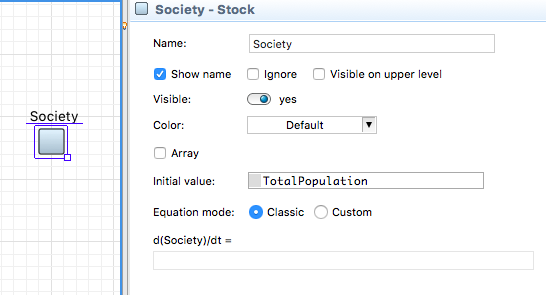
\includegraphics[height=0.3\textwidth]{img/screens/society/society1}
  \caption{The Society stock and its properties}
\end{figure}

The parameters that we were using in previous chapters will help to define the initial value for Society, too. TotalPopulation is a parameter, which will have a symbolic value of 100000. This is an approximation of a small town population.

\begin{figure}[H]
  \centering
  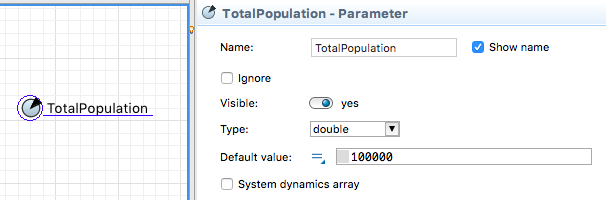
\includegraphics[height=0.3\textwidth]{img/screens/society/society2}
  \caption{The setting of TotalPopulation parameter}
\end{figure}

In order to use the TotalPopulation parameter in the Society stock value, we need to draw some connection between them. This is the way we used to bind parameters to other objects, like stocks.

\begin{figure}[H]
  \centering
  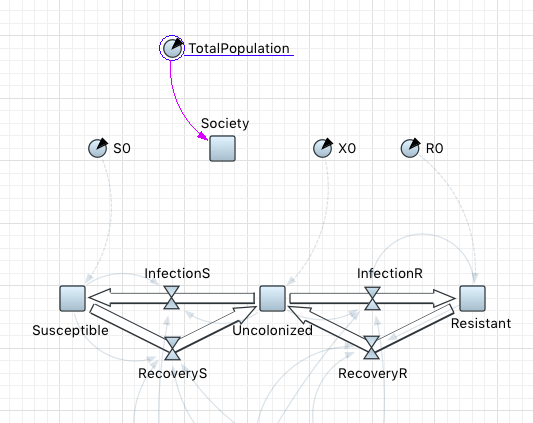
\includegraphics[height=0.5\textwidth]{img/screens/society/society3}
  \caption{Linking the Society and TotalPopulation in the model}
\end{figure}
